\paragraph{QuizziPedia::Front-End::Models::UserDetailsModel}
		
		\label{QuizziPedia::Front-End::Models:.UserDetailsModel}
		
		\begin{figure}[ht]
			\centering
			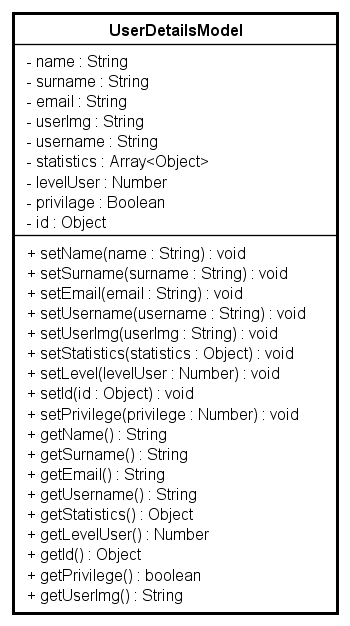
\includegraphics[scale=0.5,keepaspectratio]{UML/Classi/Front-End/QuizziPedia_Front-end_Models_UserDetailsModel.png}
			\caption{QuizziPedia::Front-End::Models::UserDetailsModel}
		\end{figure} \FloatBarrier
		
		\begin{itemize}
			\item \textbf{Descrizione}: rappresenta un utente. Contiene tutte le informazioni necessarie alla presentazione del contenuto di un utente sia nella visualizzazione che nella gestione di un profilo;
			\item \textbf{Utilizzo}: viene utilizzata per memorizzare i dati di un utente;
			\item \textbf{Relazioni con altre classi}: 
			\begin{itemize}
				\item \textbf{OUT} \texttt{LoginController}: questa classe permette di gestire l'autenticazione dell'utente al sistema;
				\item \textbf{OUT} \texttt{SearchController}: questa classe permette di gestire la ricerca di questionari e utenti all'interno dell'applicazione;
				\item \textbf{OUT} \texttt{UserDetailsController}: questa classe permette di gestire i dati di un utente;
				\item \textbf{OUT} \texttt{StatisticsController}: questa classe permette di le statistiche di un utente.
			\end{itemize}
			\item \textbf{Attributi}: 
			\begin{itemize}
				\item 
				\texttt{- name: String}\\
				Rappresenta il nome  dell'utente registrato;
				\item 
				\texttt{- surname: String}\\
				Rappresenta il cognome  dell'utente registrato;
				\item 
				\texttt{- email: String}\\
				Rappresenta l'email  dell'utente registrato;
				\item 
				\texttt{- userImg: String}\\
				Rappresenta il path della foto profilo dell'utente registrato;
				\item 
				\texttt{- username: String}\\ 
				Rappresenta l'username con cui viene identificato l'utente all'interno dell'applicazione;		  		
				\item
				\texttt{- statistics: Array<Object>}\\
				Contenente i seguenti attributi:
				\begin{itemize}
					\item
					\texttt{- topicName: String}\\
					Rappresenta il nome della statistica relativa all'argomento;	 
					\item
					\texttt{- topicLevel: Number}\\
					Identifica il livello di preparazione dell'utente in un determinato argomento;
					\item
					\texttt{- correctAnswers: Number}\\
					Identifica il numero di risposte corrette date dall'utente riguardanti domande di un determinato argomento; 
					\item						
					\texttt{- totalAnswers: Number}\\
					Identifica il numero di risposte totali date dall'utente riguardanti domande di un determinato argomento.		
				\end{itemize}		
				\item 
				\texttt{- levelUser: Number}\\
				Identifica il livello dell'utente;			
				\item 
				\texttt{- privilege: Boolean}\\
				Identifica la tipologia dell'utente;	
				\item
				\texttt{- id: Object}
				Identifica l'\texttt{id} dell'utente;
			\end{itemize}
			\item \textbf{Metodi}: 
			\begin{itemize}
				\item \texttt{+ setName(name: String): void} \\
				Metodo \textit{setter\ped{G}} per il campo dati \texttt{name}.\\
				\textbf{Parametri}:
				\begin{itemize}
					\item {name: String}\\
					Questo parametro contiene il nome dell'utente.
				\end{itemize}
				
				\item \texttt{+ setSurname(surname: String): void} \\
				Metodo \textit{setter\ped{G}} per il campo dati \texttt{surname}.\\
				\textbf{Parametri}:
				\begin{itemize}
					\item {surname: String}\\
					Questo parametro contiene il cognome dell'utente.
				\end{itemize}
				
				\item \texttt{+ setEmail(email: String): void} \\
				Metodo \textit{setter\ped{G}} per il campo dati \texttt{email}.\\
				\textbf{Parametri}:
				\begin{itemize}
					\item {email: String}\\
					Questo parametro contiene l'indirizzo email dell'utente.
				\end{itemize}
				
				\item \texttt{+ setUsername(username: String): void} \\
				Metodo \textit{setter\ped{G}} per il campo dati \texttt{username}.\\
				\textbf{Parametri}:
				\begin{itemize}
					\item {username: String}\\
					Questo parametro contiene lo username dell'utente.
				\end{itemize}
				
				\item \texttt{+ setUserImg(userImg: String): void} \\
				Metodo \textit{setter\ped{G}} per il campo dati \texttt{userImg}.\\
				\textbf{Parametri}:
				\begin{itemize}
					\item {userImg: String}\\
					Questo parametro contiene l'url dell'immagine profilo dell'utente.
				\end{itemize}
				
				\item \texttt{+ setStatistics(statistics: Object): void} \\
				Metodo \textit{setter\ped{G}} per il campo dati \texttt{statistics}.\\
				\textbf{Parametri}:
				\begin{itemize}
					\item {statistics: Object}\\
					Questo parametro contiene le statistiche dell'utente.
				\end{itemize}
				
				\item \texttt{+ setLevel(levelUser: Number): void} \\
				Metodo \textit{setter\ped{G}} per il campo dati \texttt{userLever}.\\
				\textbf{Parametri}:
				\begin{itemize}
					\item {levelUser: Number}\\
					Questo parametro contiene il livello dell'utente.
				\end{itemize}
				
				\item \texttt{+ setId(id: Object): void} \\
				Metodo \textit{setter\ped{G}} per il campo dati \texttt{id}.\\
				\textbf{Parametri}:
				\begin{itemize}
					\item {id: ObjectId}\\
					Questo parametro contiene l'id dell'utente.
				\end{itemize}
				
				\item \texttt{+ setPrivilege(privilege: Number): void} \\
				Metodo \textit{setter\ped{G}} per il campo dati \texttt{privilege}.\\
				\textbf{Parametri}:
				\begin{itemize}
					\item {privilege: Number}\\
					Questo parametro rappresenta la tipologia di utente.
				\end{itemize}
				
				\item \texttt{+ getName(): String} \\
				Metodo \textit{getter\ped{G}} che restituisce il campo dati \texttt{name};
				
				\item \texttt{+ getSurname(): String} \\
				Metodo \textit{getter\ped{G}} che restituisce il campo dati \texttt{surname};
				
				\item \texttt{+ getEmail(): String} \\
				Metodo \textit{getter\ped{G}} che restituisce il campo dati \texttt{email};
				
				\item \texttt{+ getUsername(): String} \\
				Metodo \textit{getter\ped{G}} che restituisce il campo dati \texttt{username};
				
				\item \texttt{+ getStatistics(): Object} \\
				Metodo \textit{getter\ped{G}} che restituisce il campo dati \texttt{statistics};
				
				\item \texttt{+ getLevelUser(): Number} \\
				Metodo \textit{getter\ped{G}} che restituisce il campo dati \texttt{levelUser};
				
				\item \texttt{+ getId(): Object} \\
				Metodo \textit{getter\ped{G}} che restituisce il campo dati \texttt{id};
				
				\item \texttt{+ getPrivilege(): boolean} \\
				Metodo \textit{getter\ped{G}} che restituisce il campo dati \texttt{privilege};
				
				\item \texttt{+ getUserImg(): String} \\
				Metodo \textit{getter\ped{G}} che restituisce il campo dati \texttt{userImg};
				
			\end{itemize}
		\end{itemize}	
		
		